\documentclass{scu-thesis}
 \usepackage{graphicx}	% for including graphics
% \usepackage{amsmath}	% for advanced typesetting of mathematics
% \usepackage{txfonts}	% for using the Times-Roman font
% \usepackage{natbib}	% for better citation styles

\graphicspath{{/Users/Me/Documents/github/latex-sd/images/}}

% These must be set first ... the rest of the thesis commands rely on them.

\author{Karsten Andersen}
\author{Matt Gibson}
\title{On the Relative Positioning of Mobile Devices Through Bluetooth Analysis}
\department{Department of Computer Engineering}
\degree{Bachelor of Science in Computer Science and Engineering}


% Only bachelor's theses should have multiple authors and/or be from
% multiple departments.  Signatures required:
%
% Bachelor's theses: advisor(s), department chair(s)
% Master's theses: advisor, reader, department chair
% Doctoral theses: doctoral committee (including advisor), department chair

\begin{document}
\frontmatter
\signature{Thesis Advisor}
\signature{Thesis Advisor}
\signature{Department Chair}
\signature{Department Chair}

\maketitle
\begin{abstract}

Currently, there is no way to accurately track a mobile device’s position in a given space without the use of GPS or WiFi.
This means that people who are interested in understanding where they currently are in relationship to other people or landmarks and do
not have access to these technologies are not able to get accurate location information. In many cases, GPS and WiFi fail to provide the
accuracy required to provide useful information as well.
\newline \par
Our solution is a software layer that utilizes existing bluetooth
hardware to create a highly accurate relative positioning system. The software layer will utilize a variety of algorithms to interpret the
relative signal strength of known bluetooth transmitters and will be able to return a useful, three dimensional, representation of
where a smartphone or other bluetooth device is. The framework offers a software solution that will be cheap and
highly distributable due to the fact that it utilizes existing technologies.

\end{abstract}


\tableofcontents
\listoffigures

\mainmatter
\chapter{Introduction}

\section{Motivation}

Currently, there is no way to accurately track a mobile device’s position in a given space without the use of GPS or WiFi.
This means that people who are interested in understanding where they currently are in relationship to other people or landmarks and do
not have access to these technologies are not able to get accurate location information.
While most people with modern smartphones do have nearly unlimited access to GPS and WiFi, this does not necessarily exclude them
from the group of people who are affected by this issue.  In many cases, GPS and WiFi fail to provide the fine grain accuracy required
to provide useful information.  Within a building GPS and WiFi can be unreliable because their physical signature is fundamentally not
designed to address the need for indoor or finely tuned positioning. This can cause the distance and elevation that GPS reports back to
lose accuracy. It cannot determine what floor you’re on so if you’re on the second floor or the ninth floor, you would show up in the
same location. In terms of distance, it could show you at least several meters off from your real world location.
Best case scenario, GPS will get someone to the door of a building they are looking for, but after that the person is on their own once
inside of that building. Due to their design, GPS and WiFi cannot help you determine your location once inside a building in many cases,
especially if the building has multiple floors. Often times stores and campuses provide physical maps for visitors. For a physical map
however, there is no map for finding the map. To use the map, a person physically has to move to it to view where they are. Also, if
there is a single map for all visitors, then a person can’t carry it with them once they head for their destination. This means people
can get lost on the way to their destination after leaving the map. Other current solutions try to solve this issue with proximity
detection technology. The problem here is that proximity based systems can only tell a person how close they are relative to something;
it doesn’t give information on the direction or elevation of whatever the person may be looking for. This can cause people to waste time
figuring out what direction they need to head in or even put them a floor above or below their destination.

\section{Solution}

The solution being proposed
is a software layer that utilizes existing bluetooth hardware to create a highly accurate relative positioning system.
The software layer will utilize a variety of algorithms to interpret the relative signal strength of known bluetooth transmitters
and will be able to return a useful, three dimensional, representation of where a smartphone or other bluetooth device is.
The ability to understand the location of a device in two or three dimensions as opposed to the proximity of a device in one
dimension allows for an exponential increase in the possible applications for such a positioning framework.  Additionally,
the ability to navigate using a smartphone indoors vastly improves the currently nondigital solution of central physical maps
that are currently in use in many large buildings.  The proposed framework offers a software solution that will be cheap and
highly distributable due to the fact that is utilizes existing technologies.  This means the framework will be able to support a
wide variety of applications without needing to wait around for the next breakthrough spectrum standard in positioning technology.

\begin{figure}
\chapter{Use Cases}
Displays the use case diagram and the description of each. The purpose is to define tasks an actor will perform to achieve a certain goal.
\newline
\includegraphics[width=1\textwidth]{useCaseSD.png}
\caption{Use Case Diagram}

1.
\begin{itemize}
\item Name: Install and Document Beacon Data
\item Goal: To install and load location and other info about bluetooth beacons
\item Actors: Admin/Technician
\item Preconditions:Bluetooth beacons must be placed and initialized
\item Steps: Location and other information is stored into a database
\item Post-conditions: Database will have bluetooth beacon data loaded
\item Exceptions: Information uploaded is incorrect
\end{itemize}
\end{figure}
\begin{figure}
2.
\begin{itemize}
\item Name: Use Framework for Precise Relative Location
\item Goal: To use framework to help application to discover the device's precise relative location
\item Actors: Developer
\item Preconditions:Framework must be loaded
\item Steps: Developer writes code to utilize framework
\item Post-conditions: Application will be able to discover the device's precise relative location
\item Exceptions: Framework isn't loaded or used properly
\end{itemize}
3.
\begin{itemize}
\item Name: Use Application to Find Precise Relative Location
\item Goal: To use application to discover the device's precise relative location
\item Actors: End User
\item Preconditions:Application must be downloaded
\item Steps: User opens and uses application
\item Post-conditions: End User will be able to discover the device's precise relative location
\item Exceptions: Application isn't downloaded or used properly
\end{itemize}
\end{figure}

\begin{figure}
\chapter{Activity Diagram}
The following is an activity diagrams that shows the flow of decisions being made by the framework as it encounters a location request from an app built on top of it.
\newline
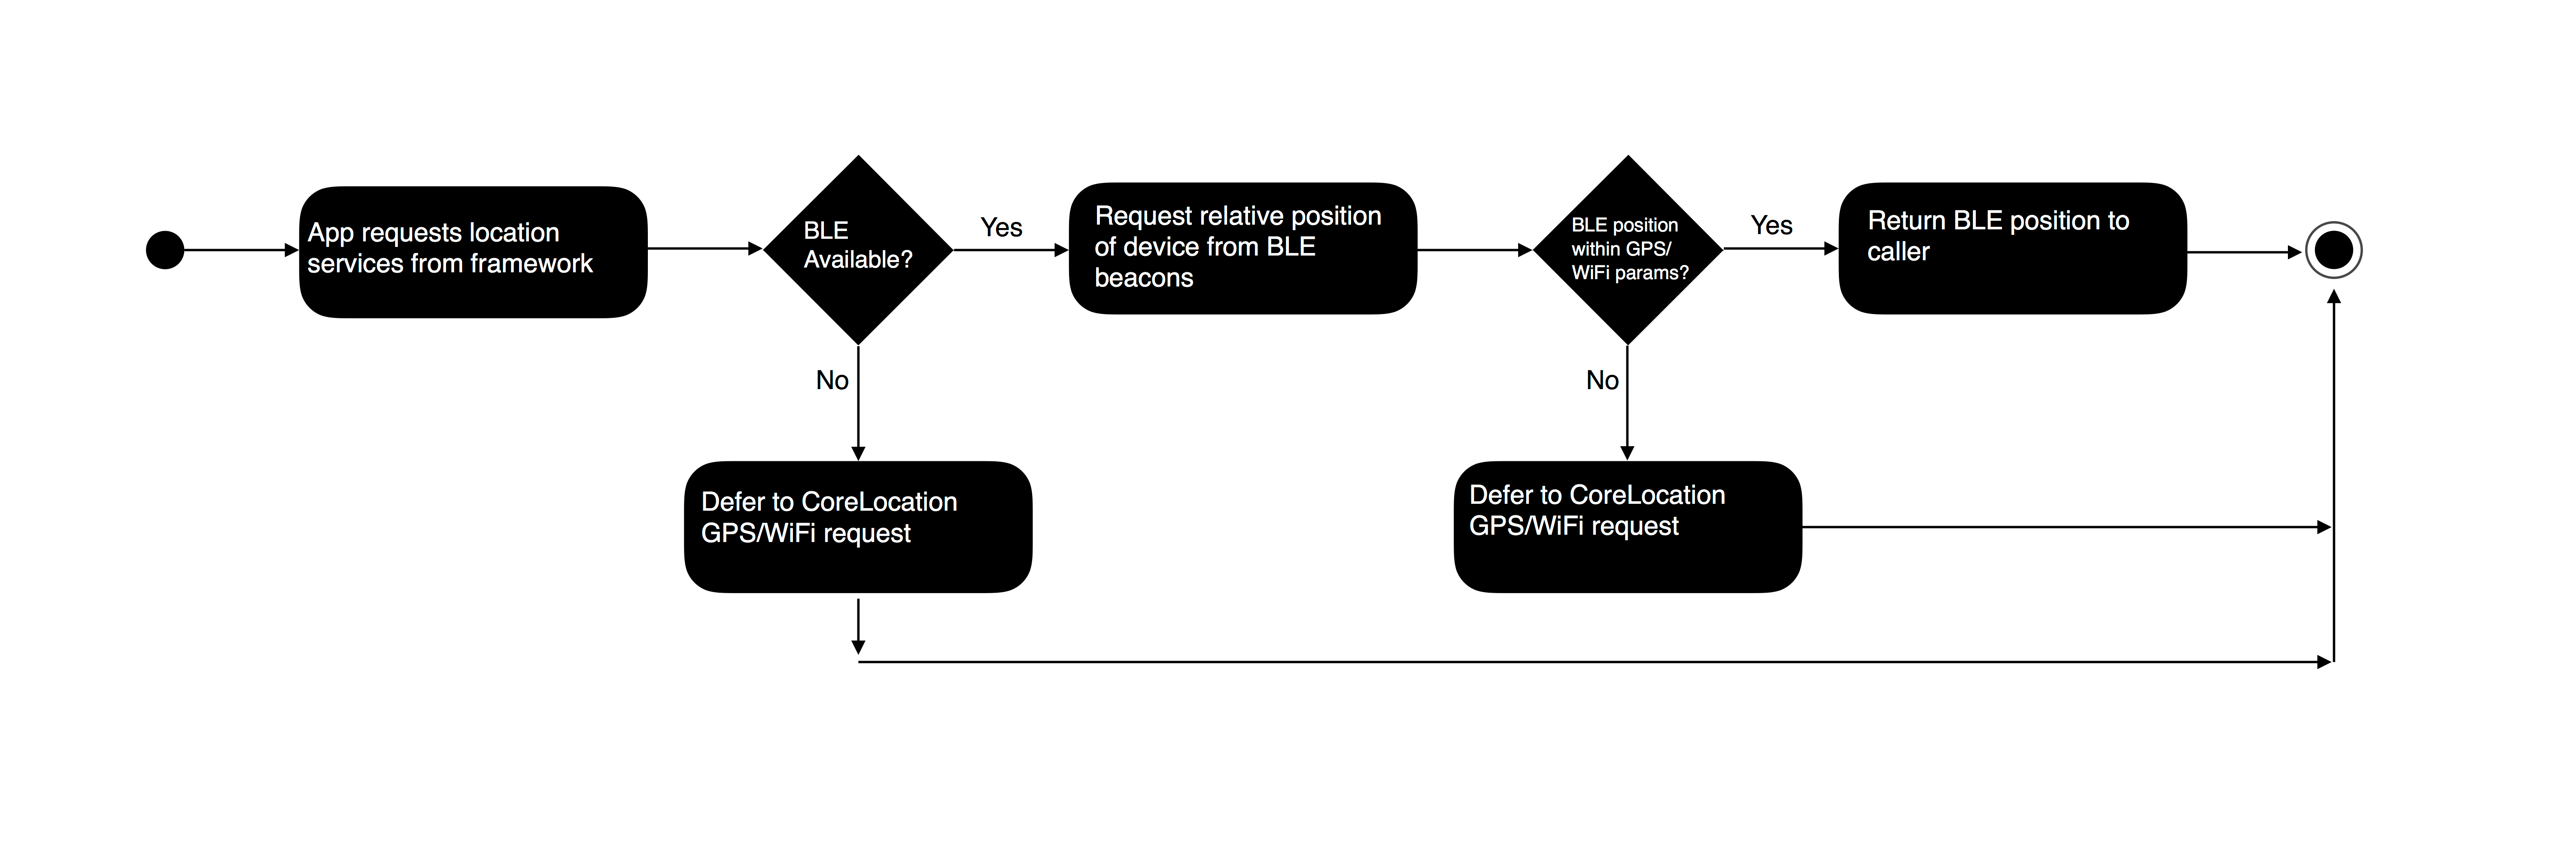
\includegraphics[width=1\textwidth]{images/act.png}
\caption{Activity Diagram}
\end{figure}

\begin{figure}
\chapter{Conceptual Model}
The conceptual model displays examples of our framework in use by an app. This specific on is taking place in a mall.
\newline
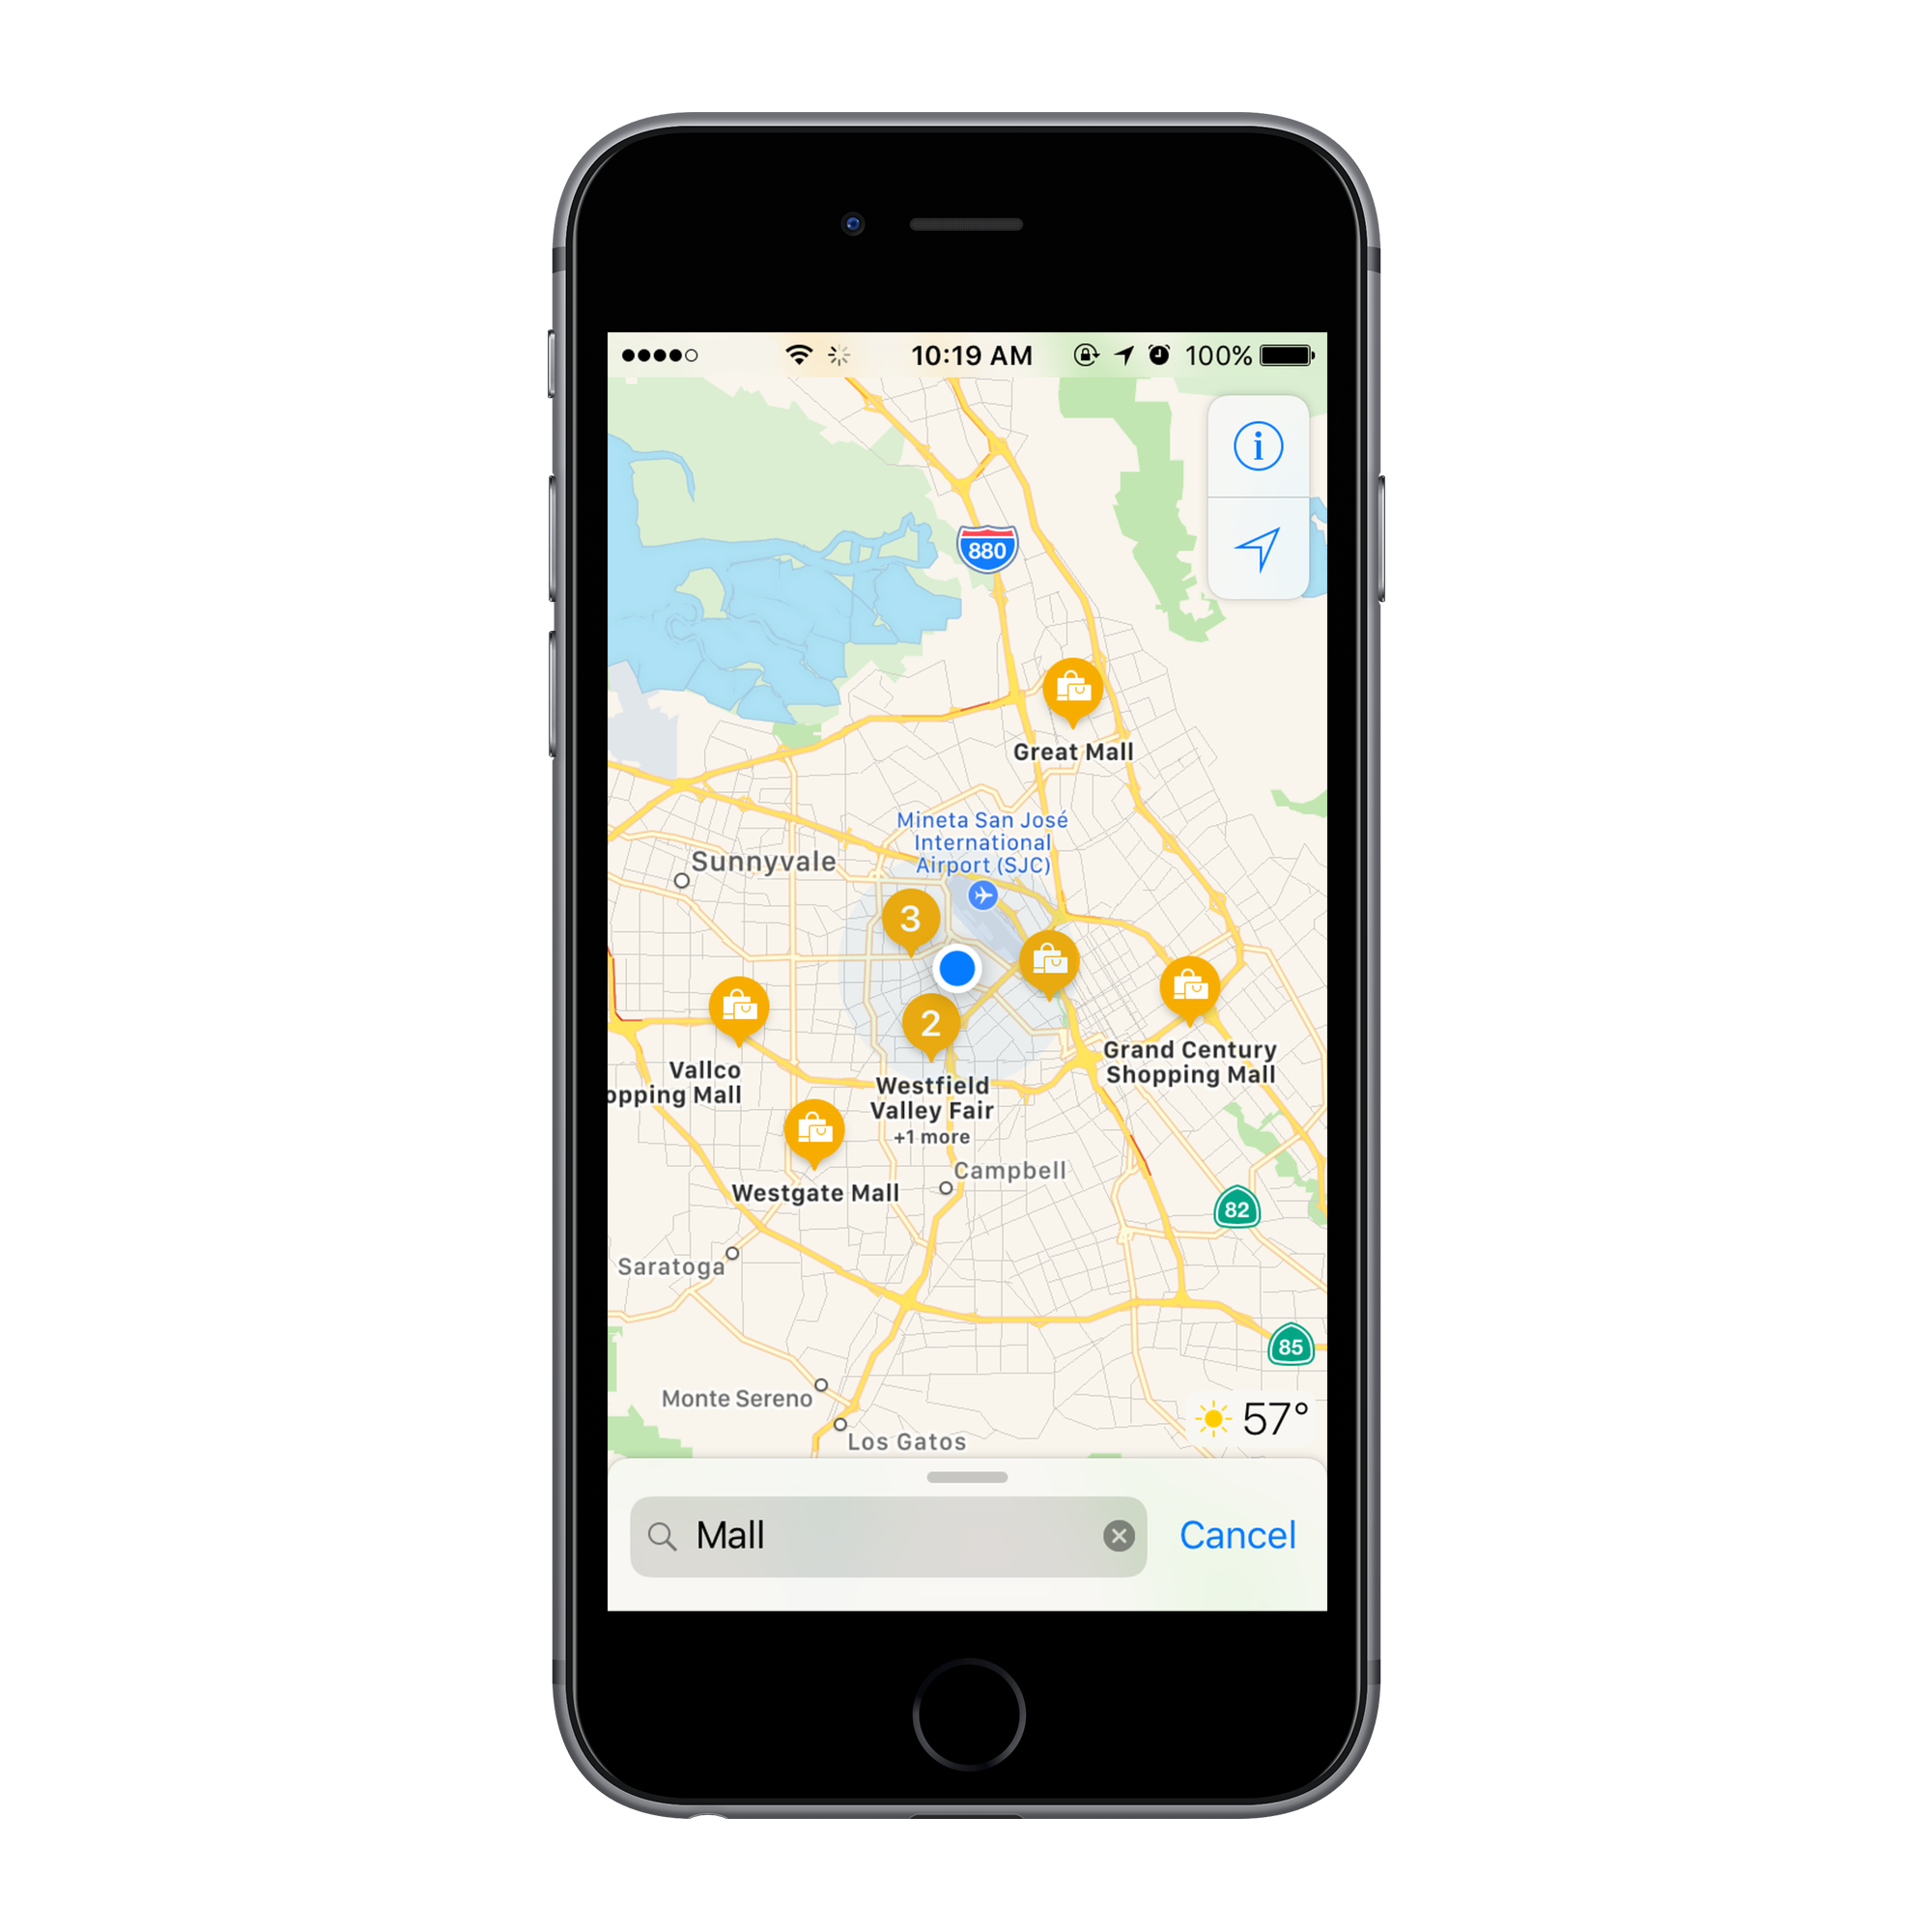
\includegraphics[width=1\textwidth]{images/con1.png}
\caption{Discovering Beacons View}
This is an example of what it would look like while the device is finding bluetooth beacons
\end{figure}
\begin{figure}
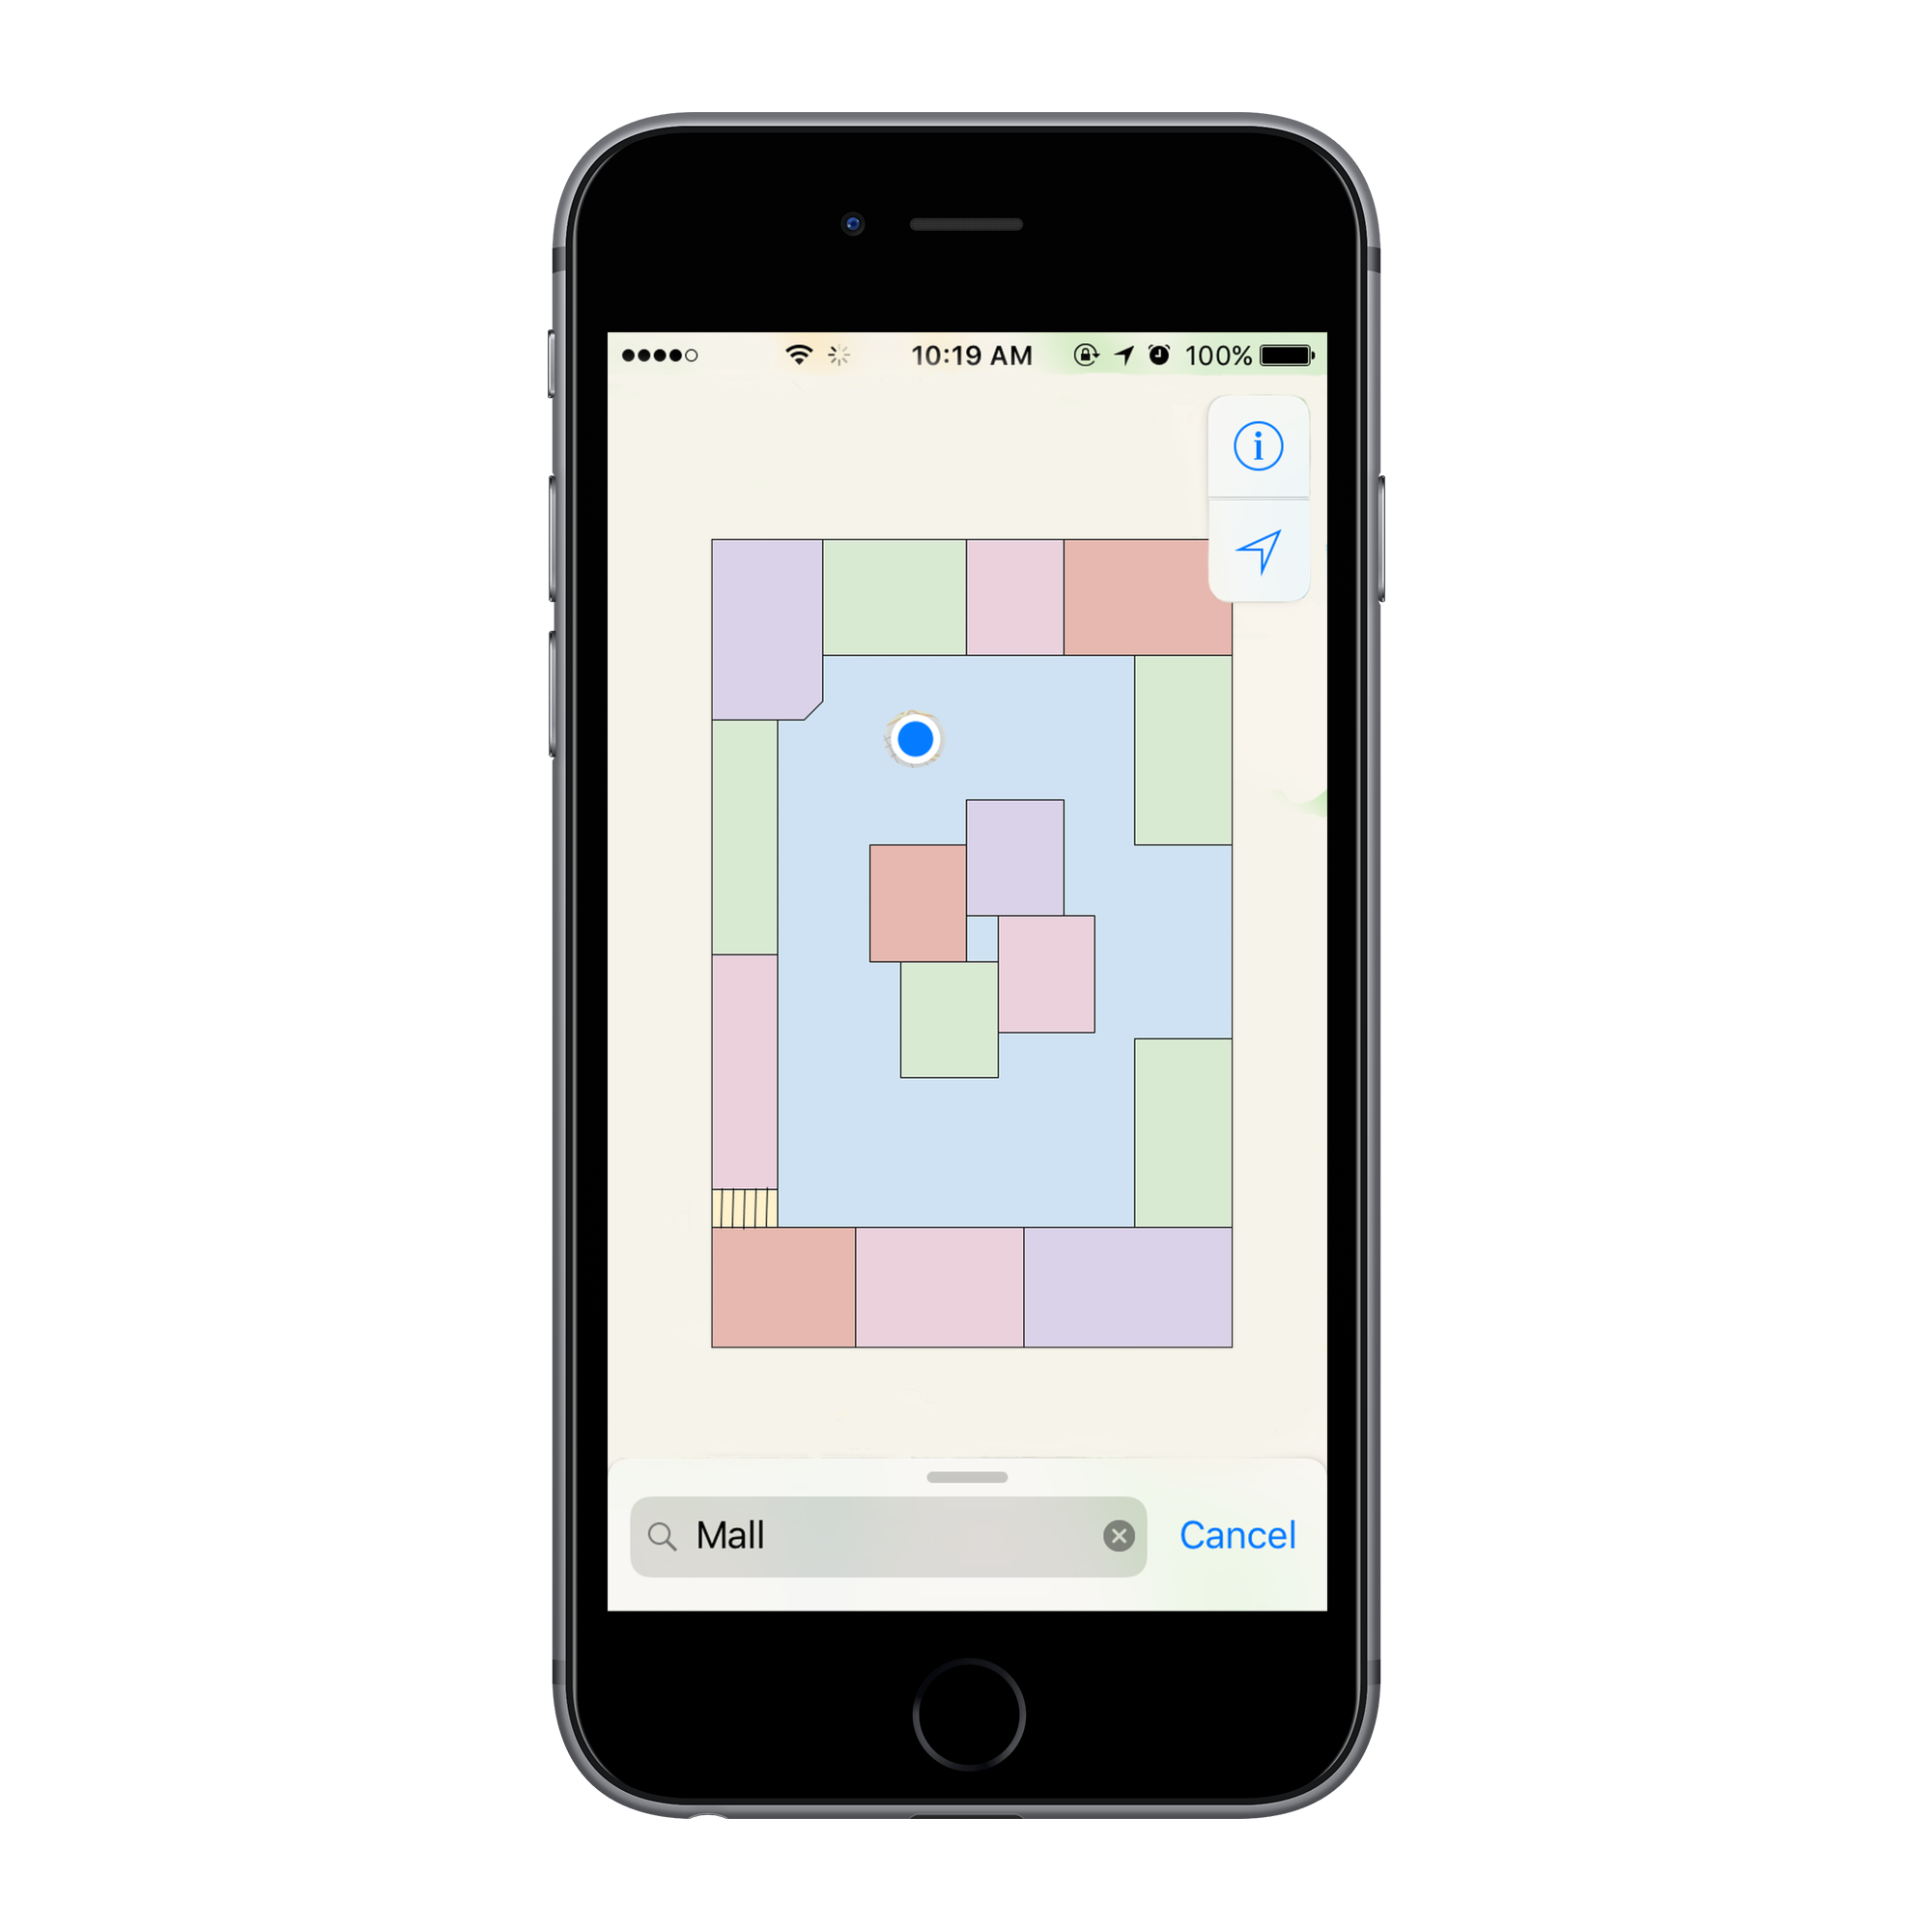
\includegraphics[width=1\textwidth]{images/con2.png}
\caption{Location View}
This is an example of what it would look like while the device is displaying relative location
\end{figure}

\chapter{Design and Implementation}

\section{Technologies Used}

Framework:

\begin{itemize}
\item Swift - Swift is the most modern language used for producing native iOS apps.  It is more readable and flexible than Obj-C, making it a better choice for this project. It is also backwards compatible with Obj-C and C++ libraries so it does not limit the usage of open source material in the system. It is used for the framework as well as the trilateration calculations.
\end{itemize}

Admin Webservice:

\begin{itemize}
\item HTML/CSS - Will be used for formatting and styling of admin webpage.
\item Javascript and JQuery - Javascript was used to add responsiveness and to provide underlying front end logic. JQuery was used to simplify DOM manipulation of admin webpage and AJAX calls.
\item PHP - Used on the back end of the admin web service to sanitize inputs and interface with the database.
\item MySQL - Used for the datastore of the admin web service.
\item Google Maps API - Used for abstract mapping of floor plan to real life latitude and longitude.
\end{itemize}

Network:
\begin{itemize}
\item iBeacon - the iBeacon protocol will be used in all broadcasting beacons
\end{itemize}

\begin{figure}
\section{Architectural Diagram}
The following architectural diagram shows that the framework conceptually is built on top of the iOS CoreLocation service.  The admin web app will only have to be reachable by the framework during the initial phase of the system installation or when major changes are made to the system.
\newline
\includegraphics[width=1\textwidth]{images/arch.png}
\caption{Architectural Diagram}
\end{figure}

\chapter{Design Rationale}
Programming Languages:
Swift is a modern and well supported language that will provide both the native support necessary and the robustness and optimization to support heavy parallel computation as well as the mathematical algorithms that require a large amount of customization and testing.

HTML, CSS, Javascript, PHP, and mySQL are all industry standard and well tested and documented.  This makes them the obvious choice to implement the web interface for the admin portal.
\newline
Architecture:
Building the framework on top of the existing CoreLocation framework in iOS provides a level of abstraction to developers who want to use precise location services without needing to know the details of that hardware system is providing the data.  While conceptually the framework is built on top of CoreLocation, in practice it would be more accurate to say it extends CL.  This means that developers who do want to fine tune the way they use the BLE Positioning Framework will be able to do so.  

Hosting the configuration portal for the system as a web service provided over the Internet have potential drawbacks (needing an Internet connection at some points limits certain geographical regions).  However, the initial positioning data of given beacon sets needs to be stored somewhere, and a central web server is much safer than a distributed system which leans more heavily on the competence of the end user.

\begin{figure}
\chapter{Risk Analysis}
The Risk Analysis table defines a potential set of risks that our group determined were possible to face, as setbacks to timely progression towards our finished project. For each risk, there are two potential consequences, a probability value 0 to 1, a severity value 0 to 10, an impact value (impact=probability*severity), and potential mitigation strategies.
\newline
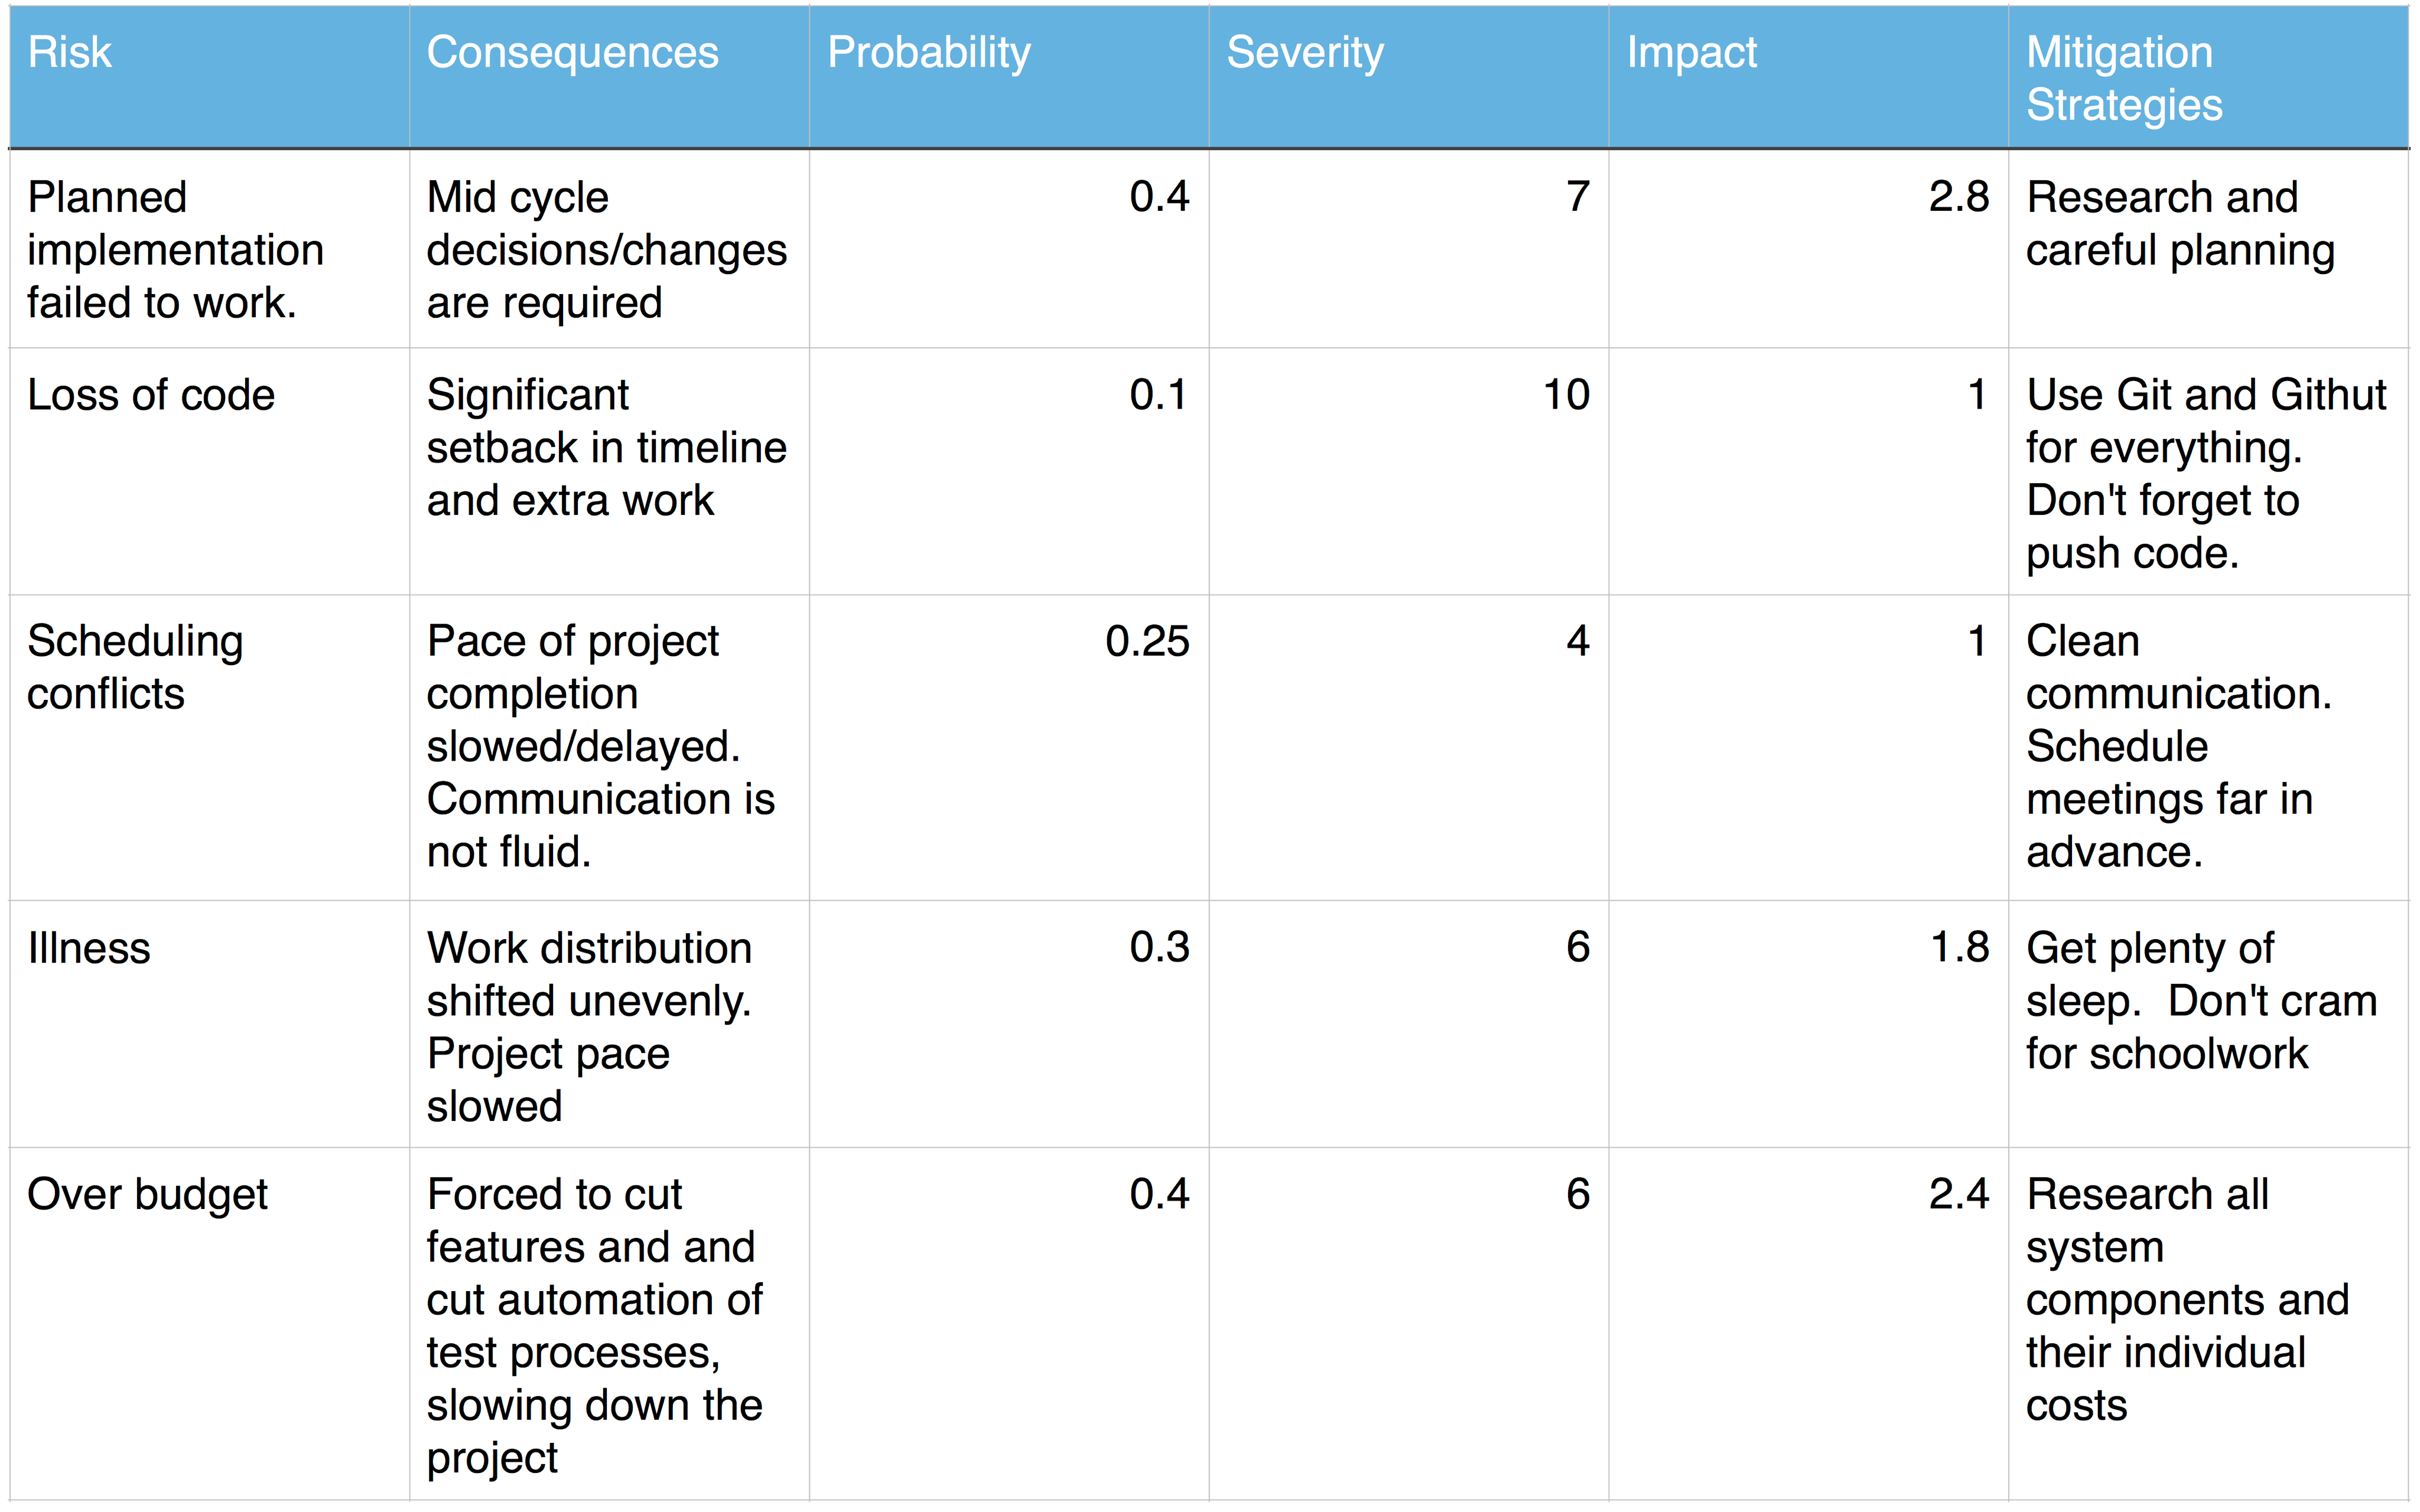
\includegraphics[width=1\textwidth]{images/risk.png}
\caption{Risk Analysis Table}
\par The two most potentially impactful risks are if the planned implementation of the system failed to provide good results, and if the project runs over budget.  By coding in a modular style that provides low coupling, the system can be modified if necessary without having to start from scratch.  Additionally, by buying most line items in the budget up front, we can be sure that the costs do not balloon as the project progresses.
\end{figure}

\begin{figure}
\chapter{Development Timeline}
The Development Timeline is a graphical representation of all the tasks that are needed for the completion of the project. This graphical model is known as Gantt Chart.
\newline
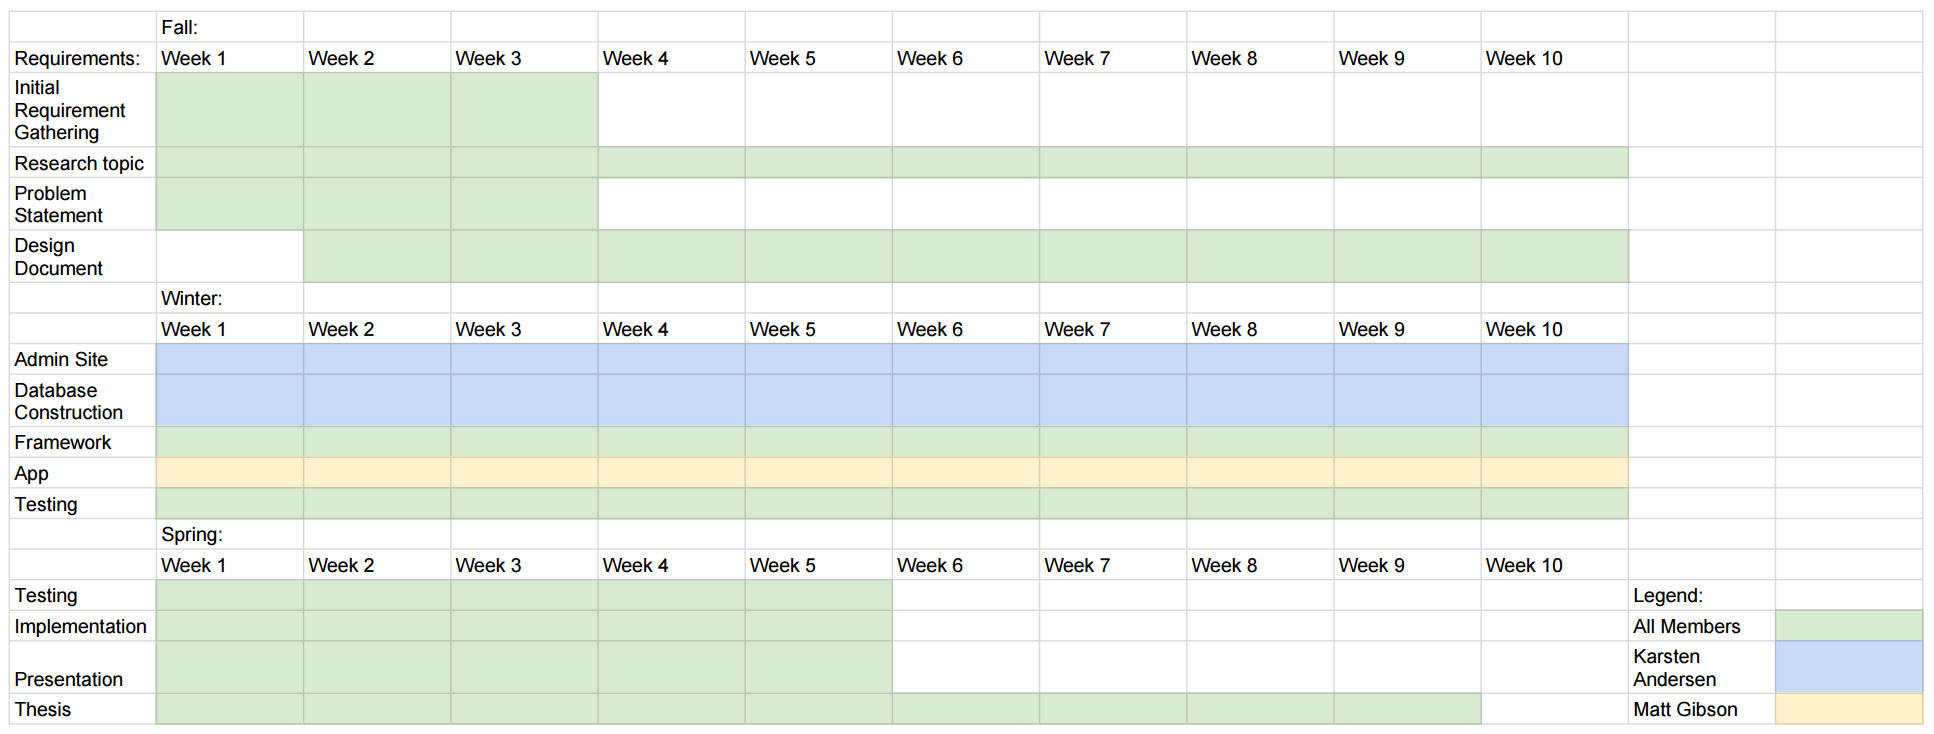
\includegraphics[width=1\textwidth]{images/gantt.png}
\caption{Gantt Chart}
The table columns in the Gantt Chart lists the set time periods over which the project is distributed in. For our purpose, we have divided the project across ten weeks for each quarter. The rows of the table in the chart lists the various tasks that need to completed. The intersection of the rows and columns in the Gantt Chart would provide data about the team member who will be working on a respective task and when a particular task is due for submission or presentation.
 The Gantt Chart proves to be an efficient visual method of tracking the different tasks of the project and helps staying on schedule.
\end{figure}

\chapter{Testing and Results}
\begin{itemize}
\item
Unit Testing: Most testing will be done by our developers using manual white box testing. Automated testing will not be used because it would not give us the desired results and will take as much time setting up as it would do to just test manually.

	We will start off with General Feature Testing wherein we will code a particular feature and test it for it's functionality. As the Unit Testing model recommends, every time we write a new feature, we will test it for its functionality ensuring minimization of errors.
    This method will help us break our system into smaller, more manageable parts, the testing of which will be relatively simpler. It will also help us make these small parts ready to be used as a part of the bigger system.
\end{itemize}

\begin{itemize}
\item Regression Testing: As we will progress with the development of the system, we will begin implementing Regression Tests on top of the general feature testing. Unlike what we will do in Unit Testing, in Regression Testing we will write and test a particular feature and test the system. Once everything works fine, we will add the next feature and then retest the system from the beginning, instead of just testing the new feature.

Simply put, regression testing is testing the system in its entirety every time a change or addition is made to it to make sure the already implemented features are not be affected by the new features in an undesirable way.

Regression testing will help us efficiently manage our system whenever a change will be made.
\end{itemize}
\begin{itemize}
\item Ad hoc Testing: Ad hoc testing is performed without a plan of action. It will be performed by improvisation where the testers will find bugs by any means that seemed appropriate. Ad hoc tests will help us spot out any strange bugs that could arise in the operation of the system.
\end{itemize}

\chapter{Ethical Analysis}
\begin{itemize}
\item Ethical
\begin{itemize}
\item There are no real ethical questions because there is no outcome that could have an immoral aspect.
\end{itemize}
\item Social
\begin{itemize}
\item This could have an impact on society because it could decrease the amount of time people spend at malls or other places due to more efficient navigation of a building. People might spend less time in public, will less likely run into people at the mall or other places, and overall reduce person-to-person contact. It could also reduce the amount of impromptu purchases from businesses because people will not have to walk by unnecessary stores.
\end{itemize}
\item Political
\begin{itemize}
\item There are no real political questions because this will not affect government at any level besides maybe easier navigation in their buildings.
\end{itemize}
\item Economic
\begin{itemize}
\item The cost of development will be relatively low because iBeacons are inexpensive, easy to maintain, and the framework can be reproduced as many times as you want for no extra cost.
\end{itemize}
\item Health and Safety
\begin{itemize}
\item There are no real risks to Health and Safety questions because bluetooth is safe for public use.
\item A potential benefit is that it could allows Emergency Medical Services to quickly navigate buildings to have a better response to a critical situation.
\end{itemize}
\item Manufacturability
\begin{itemize}
\item iBeacons are an existing product and the framework requires no manufacturing.
\end{itemize}
\item Sustainability
\begin{itemize}
\item iBeacons' batteries can be sustained for several years on average so they won't need to be replaced very often.
\end{itemize}
\item Environmental Impact
\begin{itemize}
\item There will be minimal waste but once an iBeacon dies it will need to be recycled.
\end{itemize}
\item Usability
\begin{itemize}
\item Our framework will be easy to use for developers to help them design excellent applications.
\end{itemize}
\item Lifelong learning
\begin{itemize}
\item This project will help our group to continually learn how to gain knowledge outside a traditional lecture.
\end{itemize}
\item Compassion
\begin{itemize}
\item This project has a compassionate side because it will help reduce the stress for developers creating location based apps and reduce stress for users when navigating inside buildings.
\end{itemize}
\end{itemize}


\backmatter
\end{document}
